\section*{3. Method: federated evidence-guided research}
\subsection*{3.1 Two levels of model improvement}
The research object is an executable design $a$. A task adapter fixes the writable source interface, trainer, evaluation roles and resource budget. For predictor $f_{a,w}$, research has two levels:
\[
 w_a^{\mathcal K}=\operatorname{Fit}(a,\{D_i\}_{i\in\mathcal K}),
 \qquad
 a_{t+1}=\operatorname{Retain}(a_t,\widetilde a_t,E_t),
\]
where $\mathcal K$ denotes participating clients, $\widetilde a_t$ a proposed source change, and $E_t$ its measured development evidence. The inner procedure learns task weights; the outer procedure changes the representation, interaction module or policy. Fixed-predictor program search changes the prediction rule without new weight fitting. The research LLM remains fixed.

\begin{figure}[t]
\centering
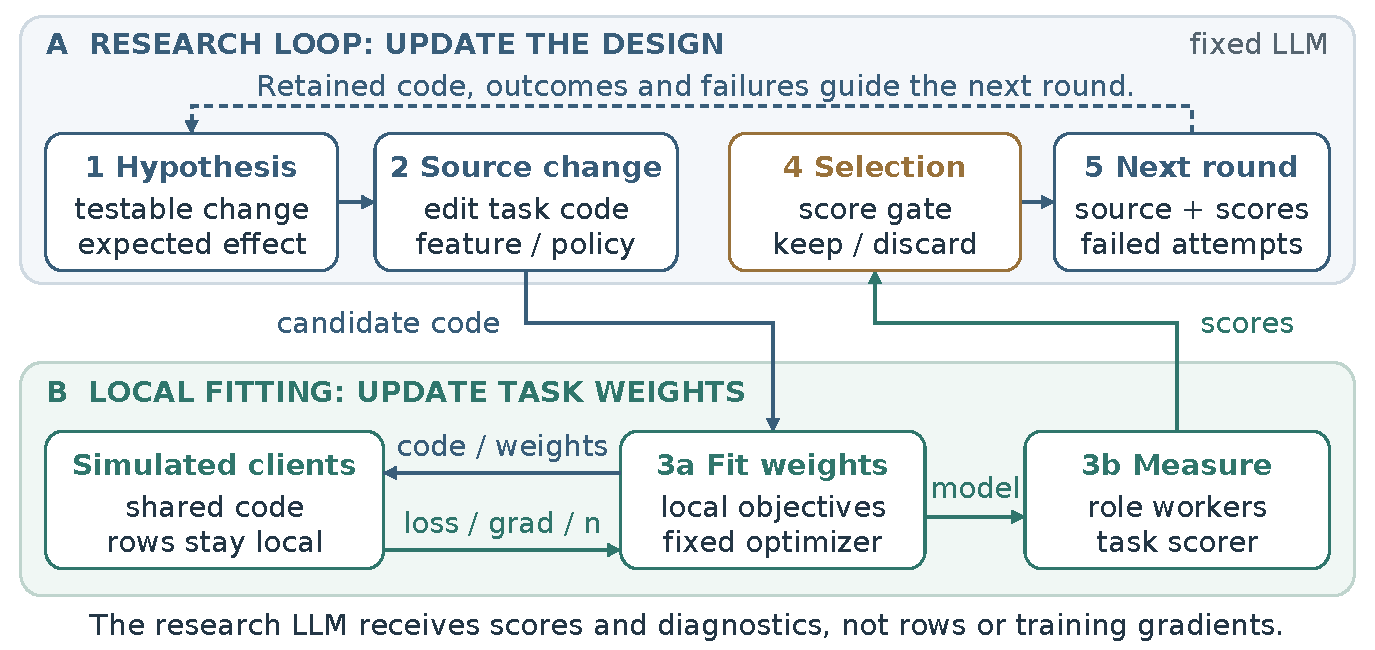
\includegraphics[width=\linewidth]{assets/method_diagram.pdf}
\caption{End-to-end pipeline. (A) Hypothesize, implement, evaluate, retain and revise. (B) Simulated clients keep separate response datasets and return gradients (proteomics) or fitted head weights (cell pilots); only evaluation summaries reach the LLM. (C) Task adapters share the research interface, not their training mode or metrics. DTI remains a centralized training/transfer study.}
\label{fig:research-interface}
\end{figure}

\subsection*{3.2 Hypotheses become measured source changes}
At round $t$, the proposer uses the task contract, shared agenda, retained source and scores, and accepted/rejected/failed history to state one change, its rationale and expected effect. Implementation edits only permitted source; interface checks precede fitting and scoring, and repairs consume the common budgets. Rejection updates the evidence, not the incumbent: subsequent proposals can learn from a failed change without inheriting it.

Retention requires both declared criteria to improve by more than $10^{-4}$: development/gate AP for the initial proteomics study, pooled out-of-fold/minimum-fold AP for its CV revision, and two validation-half AUROCs for fixed-predictor DTI. Native assessments cannot override this numerical selector. Harness-free generation uses the same task and selector but emits candidates directly, without separate hypothesis, implementation, review or memory stages.

Measured native loop attempts link hypothesis, source diff, parent, evaluator receipt, scores and decision. Failures inform subsequent proposals through separate receipts and need not appear in matched measurement history. These links expose what ran, why it was retained and which source was inherited. Native direct candidates omit separate hypotheses. The new bounded cell prototype instead shares a proposal format and varies feedback access (Appendix Q). Source inspection establishes the computation; measured outcomes, not the LLM's explanation, test its effect.

\subsection*{3.3 Local training and evidence transfer}
In the proteomics training adapter, $a$ specifies a stateless feature map $\phi_a$. Each client evaluates it on local protein responses and compound features. With $z=w^\top\phi_a(x)+b$, the fixed inner objective is logistic loss with coefficient penalty:
\[
 F_a(w,b)=\frac{1}{N}\left[\sum_{i\in\mathcal K}\sum_{(x,y)\in D_i}
 \bigl\{\log(1+e^z)-yz\bigr\}+\frac{\|w\|_2^2}{2C}\right],
 \quad N=\sum_{i\in\mathcal K}|D_i|,\ C=1.
\]
The coordinator aggregates local losses, gradients and counts for fixed L-BFGS-B updates (Figure~\ref{fig:research-interface}B). Source specifies \emph{what to fit}; client replies determine \emph{the weights}; evaluation summaries determine \emph{what to revise}. Evaluation workers receive source and fitted parameters and return aggregate scores. Training RPCs exclude raw arrays; the LLM receives neither rows nor gradients. For fixed source and clients, additivity recovers the centralized objective and gradient; Appendix K verifies equivalence. This existing optimizer lets research test changing representations with local data.

The historical evidence-only adapters instead train centrally and use partner diagnostics without adding partner training examples. Appendices C and N distinguish those studies from actual local-gradient training.

The biological motivation is access to complementary measurements under sharing constraints \citep{Sheller2020}. Direct generation receives the same client access as the loop within each condition. Crossing both controllers with one and ten clients separates research organization from data availability; fixed-feature references isolate the latter effect without source search.

\subsection*{3.4 Execution boundary}
The original source-search workers deny file opens, networking and new processes after initialization; fixed scorers, trainers and orchestration are trusted. The new cell prototype instead accepts bounded configurations and runs persistent client workers, without claiming an adversarial filesystem sandbox. It averages locally trained head parameters with FedAvg. Offline packaging simulates institutions on one host; fitting exchanges updates and scalar summaries, not raw responses. Neither implementation provides differential privacy or secure aggregation. Direct and loop arms share the boundary within each study.
